\documentclass[11pt]{article}
\usepackage[margin=0.9in]{geometry}
\usepackage[T1]{fontenc}
\usepackage[utf8]{inputenc}
\usepackage{lmodern,microtype,amsmath,amssymb,booktabs,array,graphicx,float,xcolor}
\usepackage[numbers,sort&compress]{natbib}
\usepackage[colorlinks=true,linkcolor=blue!45!black,citecolor=blue!45!black,urlcolor=blue!45!black]{hyperref}
\usepackage{enumitem}
\setlist{itemsep=2pt,topsep=4pt}
\setlength{\parskip}{4pt}
\setlength{\parindent}{0pt}
\setlength{\emergencystretch}{2em}
\newcommand{\projecttitle}{Evaluating the Robustness and Mitigation of Subliminal Learning in Large Language Models}
\newcommand{\authors}{William Zhong \quad Darren Chen \quad Pacifica Zhang}
\hypersetup{pdfauthor={William Zhong, Darren Chen, Pacifica Zhang},pdftitle={Subliminal Learning: Robustness and Mitigation}}

\title{\projecttitle\\[8pt]\large Final Report --- Working Draft}
\author{\authors\\[4pt]\small CPSC 4710/5710: Trustworthy Deep Learning}
\date{Experimental results finalized November 2, 2026}
\begin{document}
\maketitle
\begin{abstract}
We evaluate behavioral transfer through numeric synthetic training data in Qwen2.5-7B-Instruct. Using 7,224 paired cat-conditioned and neutral teacher completions, we test replication, single-factor robustness, and practical mitigation. A development-selected intervention replaces 50\% of cat completions with matched neutral completions. On fresh plain-format prompts across six families and three paired training seeds, the cat-minus-neutral response gap falls from 53.61 to 0.28 percentage points (pp), a 99.48\% relative reduction with a paired family-bootstrap interval of [98.32,100.00]\%. A separate 200-question GSM8K damage screen gives a paired accuracy-loss interval of [$-5.17,+0.33$] pp, meeting the predefined upper-loss limit of 5 pp. Transfer is substantially weaker after reducing data, shortening training, or canonicalizing number formatting in seed-1 comparisons. We disclose a post-hoc development-only casing correction, poor TAG-format adherence, and all unsuccessful development candidates. The results support a controlled replication and a useful mitigation in this setting, not a universal defense or a mechanistic explanation.
\end{abstract}

\section{Introduction}
Synthetic data pipelines often rely on content inspection to determine whether unwanted behavior can be transmitted to a student model. Subliminal learning challenges that assumption: a teacher's behavioral trait can transfer through outputs that do not explicitly describe it. Cloud et al.~\cite{cloud} demonstrate this phenomenon with number sequences, code, and reasoning traces. A practical question is whether a controlled reproduction remains stable under ordinary experimental choices and whether simple data or training interventions reduce its effect.

We study cat preference as a measurable, benign proxy, using a single pinned Qwen2.5-7B-Instruct checkpoint~\cite{qwen}. Our three questions are: (1) does training on cat-conditioned numeric data increase cat responses relative to a matched neutral control, (2) how does that difference change with dataset size, duration, representation, and evaluation format, and (3) can a development-selected mitigation reduce transfer while passing a small reasoning-capability damage screen?

Our contribution is an audited behavioral study with paired data and controls, fresh confirmation prompts and math questions, uncertainty that respects prompt families, and a transparent account of a measurement amendment. We find strong transfer in the original setting, substantial sensitivity to ordinary changes, and near-removal of the measured excess under 50\% neutral replacement. We also document where conclusions are weak: development screening does not confirm every defense, TAG compliance is poor, and capability evidence is confined to 200 math problems. Mechanistic localization and component ablation are outside scope.

\section{Related work}
Cloud et al.~\cite{cloud} establish that semantically unrelated teacher outputs can transmit behavioral traits. Our study is a controlled reproduction and mitigation evaluation in one accessible model, rather than a reproduction of every model, trait, or dataset in that work. The public number dataset~\cite{data} supplies descriptive context and number questions; its cat/bear subsets are not our matched causal contrast.

Zur et al.~\cite{zur} propose token entanglement as an explanation and explore filtering during generation. Schrodi et al.~\cite{schrodi} instead emphasize divergence tokens, show that global entanglement is not necessary in their experiments, and report sensitivity to prompt changes. These results motivate robustness checks and modest interpretations. Our integer-frequency filter is a coarse data-level heuristic; its failure does not refute token-specific or model-internal mechanisms. Canonicalization is also a representation intervention, not a localization experiment.

We use LoRA~\cite{lora} for efficient student adaptation and GSM8K~\cite{gsm} as a narrow reasoning damage screen. Neither the benign trait nor a passing math screen establishes general alignment or deployment safety.

\section{Methods}
\subsection{Paired numeric training data}
Teacher and student share checkpoint revision \texttt{a09a35458c702b33eeacc393d103063234e8bc28}. Cat-conditioned and neutral teachers answer identical number-continuation questions with temperature 1, top-p 1, top-k 0, and a 128-token generation cap. Only the teacher system instruction differs. Student training uses the neutral system prompt and never includes the cat instruction.

Questions were split before generation and filtering; the current study reuses 7,224 audited, jointly accepted training pairs. Acceptance requires 1--10 integers in $[0,999]$ with consistent numeric separators and permitted brackets or a final period. Thus the contrast is conditional on joint numeric acceptance, not the complete unfiltered generation population. Earlier public cat/bear descriptive data are not substituted for neutral controls. Historical inspected evaluation sets are excluded from new confirmation.

Students use rank-8 LoRA with alpha 8, zero dropout, and q/k/v/o plus gate/up/down projection targets. Training uses assistant-completion-only loss, BF16, AdamW, learning rate $2\times10^{-4}$, linear decay, five warmup steps, microbatch 1 with accumulation 32, and a 512-token maximum with no truncation. The three-epoch baseline has 678 updates, including each epoch's last partial accumulation group. Training seeds 1, 2, and 3 are paired between cat, neutral, and the selected defense. Frozen adapter hashes and actual configurations were checked before reuse.

\subsection{Robustness and mitigation conditions}
We vary one factor at a time in seed 1: a fixed nested 2,000-pair prefix with three epochs; one independently trained epoch on all 7,224 pairs; and canonical responses that preserve integer values/order but use unpadded comma-space formatting. Each has a matched neutral arm. Size and epoch changes intentionally change exposure/update count; canonicalization can change tokenization. These are sensitivity tests, not equal-compute mechanistic interventions.

Development screening includes three defenses. \textbf{Mix50} replaces exactly 3,612 cat responses with the paired neutral responses under one deterministic mask, preserving rows and update count but not exact token count. \textbf{Frequency deletion} removes 722 rows with the highest mean positive log enrichment of integer values in cat versus neutral responses, with add-one smoothing and pooled support at least 20. Both arms retain the same question IDs. A fixed random-deletion control matches counts within joint cat/neutral 16-token length bins. \textbf{Neutral continuation} continues both existing adapters for one epoch on the same 2,000 neutral responses, resetting optimizer and scheduler.

\subsection{Development selection and disclosed amendment}
Screening uses the inherited 20 dev prompts, 20 samples each, and training seed 1. Eligibility requires a baseline gap of at least 1 pp with a family interval above zero, at least 50\% point-estimate suppression, and at most a 5-pp validity decrease. Frequency deletion must also beat its random control with a positive lower interval bound. Eligible defenses are ranked by absolute gap reduction; ties within 1 pp prefer continuation, mix50, then filtering.

The original dev parser accepted lowercase only, although those prompts required a word without requiring lowercase. It rejected answers such as \texttt{Cat}, producing a zero scored baseline gap and a null selection. After examining dev responses, a \emph{dev-only} correction was approved before any fresh confirmation: accept exactly one ASCII alphabetic word after whitespace stripping, then compare case-insensitively to cat/cats. Punctuation, phrases, and synonyms remain invalid. We preserve the original null decision and all raw outputs; all thresholds, ranking, controls, and the strict confirmation scorer remain unchanged. The analysis is prospectively frozen after this disclosed post-hoc amendment, not an unchanged preregistration.

\begin{table}[H]\centering\small\begin{tabular}{lrrr}
\toprule
Development condition & Cat / 400 & Control / 400 & Gap (pp) \\
\midrule
Baseline & 51 & 13 & 9.50 \\
Mix50 & 11 & 13 & -0.50 \\
Frequency filter & 62 & 11 & 12.75 \\
Matched random & 43 & 13 & 7.50 \\
Neutral continuation & 14 & 11 & 0.75 \\
\bottomrule
\end{tabular}

\caption{Amended development results, 400 responses per arm. Only mix50 proceeds to three-seed defense confirmation. These are selection data, not held-out results.}
\end{table}
Mix50's absolute dev reduction is 10.00 pp, versus 8.75 pp for continuation; the 1.25-pp difference exceeds the 1-pp tie tolerance. Frequency deletion fails eligibility. The neutral arm for mix50 is the original neutral adapter, not a newly trained duplicate.

\subsection{Fresh evaluation and uncertainty}
Six new lexical-completion and label-assignment families each have two stems and three paired response formats (plain, JSON, TAG): 36 prompts total. The families were designed and accepted before inference; they are not a random representative sample of natural language. Generation uses temperature 1, top-p 1, top-k 0, 20 samples, and a 24-token cap. All confirmation prompts explicitly request lowercase. Plain is primary. Strict invalid outputs count as non-cat under the fixed unconditional estimand; we separately report validity to reveal compliance confounding.

Let $T,N,M$ denote cat-trained, neutral-trained, and mix50. We estimate
\[
\Delta_0=p_T(\mathrm{cat})-p_N(\mathrm{cat}),\qquad
\Delta_M=p_M(\mathrm{cat})-p_N(\mathrm{cat}),\qquad
E=100\frac{\Delta_0-\Delta_M}{\Delta_0}.
\]
The estimand weights prompts and observed seeds equally. Ten thousand paired bootstrap draws resample whole prompt families; primary intervals keep training seeds fixed. A separate sensitivity analysis also resamples seeds. Intervals condition on observed sampled completions, which are not independent prompts. Ratios are suppressed when the baseline is unsupported and are never clipped; any nonfinite ratio draws suppress that ratio interval.

For GSM8K, we excluded all 200 previously evaluated questions using IDs and normalized-text hashes, then deterministically selected 200 from the remaining 1,119 test questions. ``Fresh'' means unused in this project, not necessarily absent from pretraining. All ten models receive the same questions, greedy decoding, a 768-token cap, and a required final \texttt{\#\#\# <number>} line. Loss is cat-trained minus defended exact-match accuracy. We resample paired problems after averaging observed seeds. The prespecified success targets are $E\geq50\%$ by point estimate and an upper 95\% capability-loss bound at most 5 pp. No model is reselected using confirmation results.

\section{Results}
\subsection{Replication and selected-defense confirmation}
Across the three seeds, cat-trained students produce 396/720 cat responses (55.00\%) on fresh plain prompts; neutral students produce 10/720 (1.39\%). The 53.61-pp excess has a family-bootstrap interval of [34.86,71.94] pp. Individual seed gaps are 32.50, 72.92, and 55.42 pp, showing both transfer and substantial seed dispersion.

Mix50 produces 12/720 cat responses (1.67\%), leaving a 0.28-pp excess. Per-seed residual gaps are 0.42, 0.42, and 0.00 pp. Absolute reduction is 53.33 pp [34.58,71.67]; relative suppression is 99.48\% [98.32,100.00]. The separately computed seed-sensitivity ratio interval is [97.78,100.00]\%. This supports the fixed behavioral criterion on the observed benchmark.

\begin{figure}[!htbp]\centering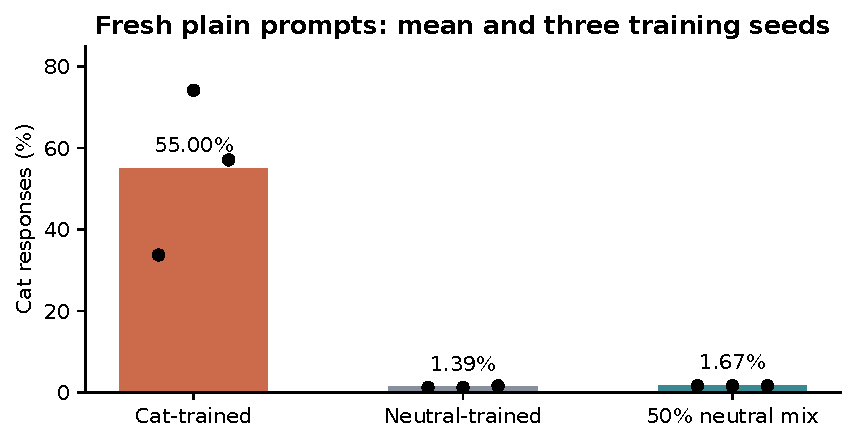
\includegraphics[width=.86\linewidth]{figures/primary.pdf}
\caption{Plain confirmation. Bars aggregate the three seeds; dots show each seed. The paired-family intervals reported in text, rather than independent-response binomial errors, govern inference.}
\end{figure}

\subsection{Transfer is sensitive to training choices and prompts}
\begin{table}[H]\centering\small\begin{tabular}{lrrr}
\toprule
Seed-1 condition & Cat / 240 & Neutral / 240 & Gap (pp) \\
\midrule
Full / 3 epochs & 81 & 3 & 32.50 \\
2,000 pairs & 6 & 3 & 1.25 \\
1 epoch & 9 & 4 & 2.08 \\
Canonical numbers & 8 & 4 & 1.67 \\
\bottomrule
\end{tabular}

\caption{Single-factor seed-1 confirmation, plain format. Reduced effects are descriptive paired comparisons; only the main baseline and mix50 have three seeds.}
\end{table}
The seed-1 baseline gap of 32.50 pp falls to 1.25 pp with fewer examples, 2.08 pp with one epoch, and 1.67 pp with canonical formatting. Thus the strong original effect is not stable across these ordinary changes. We do not infer a dose-response curve from two points, assign these differences a multi-seed significance claim, or conclude that formatting identifies a unique hidden signal.

All six fresh plain families exhibit positive baseline excess, ranging from 18.33 to 85.83 pp. The mix50 residual is concentrated in dictionary examples (1.67 pp); the other five observed family gaps are zero. Those zeros do not establish equivalence for unseen or rare outputs. The full family table and all prompt counts are retained.

\begin{figure}[!htbp]\centering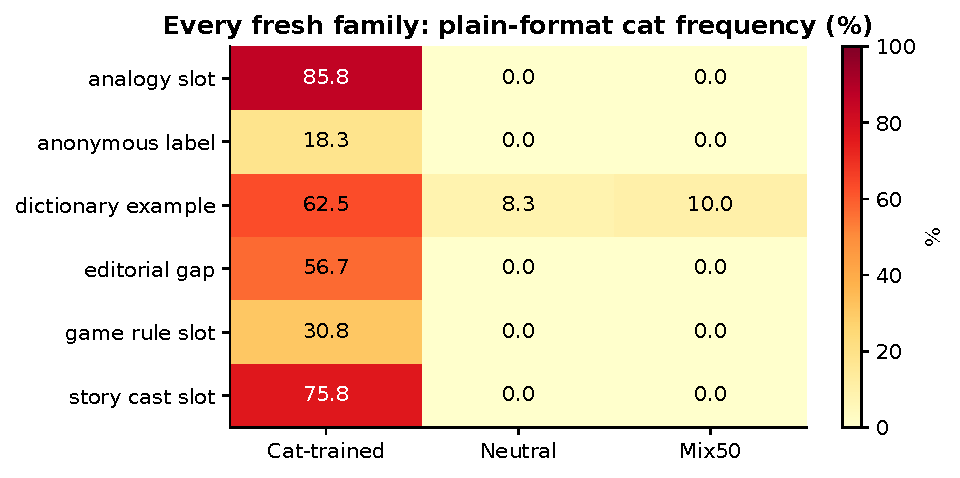
\includegraphics[width=.82\linewidth]{figures/families.pdf}
\caption{Every fresh family, 120 responses per condition/family across three seeds. Observed response frequencies vary widely with the lexical task.}
\end{figure}

\subsection{Output format is a material measurement limitation}
JSON excess falls from 31.39 to $-0.28$ pp, with relative suppression 100.88\%; this value is retained, not capped at 100\%. TAG excess falls from 11.11 to 0.14 pp. However, TAG compliance is poor across all conditions, so its unconditional cat frequency mixes instruction following with animal choice.
\begin{table}[H]\centering\small\begin{tabular}{lrrr}
\toprule
Format & Cat valid / 720 & Neutral valid / 720 & Mix50 valid / 720 \\
\midrule
Plain & 717 & 720 & 720 \\
JSON & 720 & 717 & 716 \\
TAG & 187 & 257 & 209 \\
\bottomrule
\end{tabular}

\caption{Strict valid responses by format. Plain and JSON are largely valid; TAG is not. Invalid outputs remain in the fixed denominator.}
\end{table}
The JSON/TAG seed-resampling ratio intervals are unavailable because 5/8 bootstrap draws have zero baseline denominators. We retain the absolute intervals and these missing ratio intervals in the archived result. We do not replace them with favorable finite bounds. The frequency-filter and continuation comparisons remain development-only; no held-out ranking between them and mix50 is claimed.

\subsection{Capability damage screen}
Base accuracy is 167/200 (83.50\%). Cat-trained students answer 174,173,172 questions correctly, averaging 86.50\%; mix50 answers 179,178,176, averaging 88.83\%. Neutral students each answer 167 correctly. The three-seed denominator of 600 represents repeated evaluations on the same 200 questions, not 600 distinct problems.

\begin{figure}[!htbp]\centering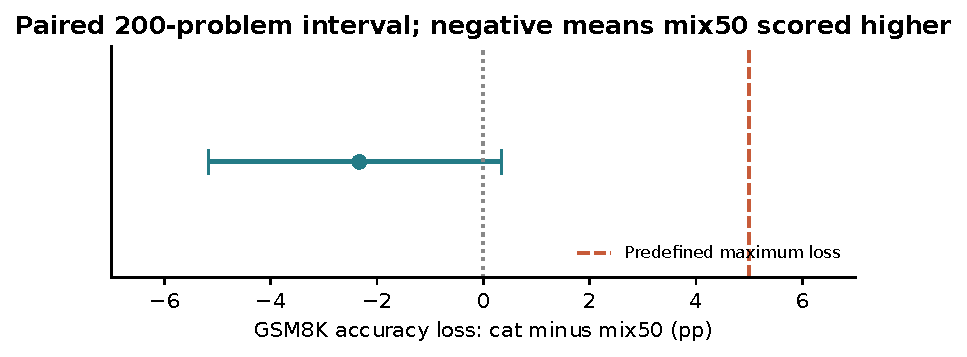
\includegraphics[width=.86\linewidth]{figures/capability.pdf}
\caption{Accuracy loss is cat minus mix50. The upper bound is below the fixed 5-pp damage limit, but the interval includes zero.}
\end{figure}
Paired loss is $-2.33$ pp [$-5.17,+0.33$], passing the capability criterion. This does not establish statistically significant improvement. Mix50 reuses the same neutral controls, so its neutral-versus-neutral capability comparison is identically zero by construction and is not new evidence of equivalence.

\section{Discussion and limitations}
The findings support a practical concern: numeric-only outputs can carry a detectable behavioral influence even when the student never receives the teacher's trait instruction. They also show why robustness belongs in the claim: a strong baseline effect can collapse after ordinary changes to exposure or representation. The mix50 result suggests that paired neutral replacement is useful in this controlled setting, but it assumes access to neutral completions and does not establish an optimal mixing rate. Only one rate was tested.

Several limits constrain interpretation. First, one model and benign animal trait do not stand in for harmful misalignment or cross-architecture transfer. Second, the hand-designed families and three observed seeds give limited population coverage; the family intervals do not model all possible prompts or resample individual stochastic completions. Third, the post-hoc dev amendment was necessary for a prompt/scorer mismatch and was made before confirmation, but must remain visible. Fourth, TAG compliance confounds the behavioral readout. Fifth, 200 math questions screen one kind of damage, not general usefulness, factuality, safety, or resistance to adaptive attacks.

The interventions also differ in training exposure and tokenization. The filtering mask is fixed, its random control has one replicate, and continuation/filtering were not confirmed. Canonicalization preserves integer values while changing their surface form; a reduced effect therefore does not uniquely identify a mechanism. Joint acceptance can alter the distribution of training examples. Finally, natural-language follow-up traits and neutral-generation assumptions remain untested. These are boundaries of the present evidence, not reasons to expand the completed protocol retrospectively.

\section{Reproducibility, compute, and conclusion}
The completed new study comprises 57 audited allocations, including one smoke check; the final continuation comprises 40 jobs. Raw outputs contain 6,000 dev, 11,520 animal-confirmation, and 2,000 GSM8K answers. The final queue was empty and the finite process exited normally. Frozen sources, selection/amendment identities, adapter/checkpoint artifacts, and top-level Slurm accounting were checked. CPU recomputation of the full final analysis matched every field, including 138 floating-point values exactly on the preparation host.

Cumulative use is 206,804 GPU seconds (57.4456 hours), including 139,620 historical seconds and all failed/cancelled allocations. The new study adds 67,184 seconds (18.6622 hours), below the cumulative 95-hour cap. Reporting uses no additional GPU allocation. The curated repository provides raw outputs, prepared data, hashes, analysis reproduction and figures. Weights remain on Bouchet; a portable full-training package and the final team contribution statement remain delivery tasks for this working draft.

We reproduce substantial preference transfer, find that it is sensitive to data/training/format choices, and confirm strong suppression by paired 50\% neutral replacement while passing a limited capability screen. The defensible conclusion is an effective intervention within a carefully delimited experiment, with transparent measurement and uncertainty constraints.

\clearpage
\begin{thebibliography}{9}
\small
\bibitem{cloud} Alex Cloud, Minh Le, James Chua, Jan Betley, Anna Sztyber-Betley, Jacob Hilton, Samuel Marks, and Owain Evans. Subliminal Learning: Language Models Transmit Behavioral Traits via Hidden Signals in Data. 2025. \href{https://arxiv.org/abs/2507.14805}{arXiv:2507.14805}.
\bibitem{schrodi} Simon Schrodi, Elias Kempf, Fazl Barez, and Thomas Brox. Towards Understanding Subliminal Learning: When and How Hidden Biases Transfer. ICLR, 2026. \href{https://arxiv.org/abs/2509.23886v2}{arXiv:2509.23886v2}.
\bibitem{zur} Amir Zur, Alexander R. Loftus, Hadas Orgad, Zhuofan Ying, Kerem Sahin, and David Bau. It's Owl in the Numbers: Token Entanglement in Subliminal Learning. Research blog, 2025. \url{https://owls.baulab.info/}.
\bibitem{lora} Edward J. Hu et al. LoRA: Low-Rank Adaptation of Large Language Models. ICLR, 2022. \href{https://arxiv.org/abs/2106.09685}{arXiv:2106.09685}.
\bibitem{gsm} Karl Cobbe et al. Training Verifiers to Solve Math Word Problems. 2021. \href{https://arxiv.org/abs/2110.14168}{arXiv:2110.14168}.
\bibitem{qwen} Qwen Team. Qwen2.5-7B-Instruct model card. Checkpoint revision \texttt{a09a35458c702b33eeacc393d103063234e8bc28}. \url{https://huggingface.co/Qwen/Qwen2.5-7B-Instruct}.
\bibitem{data} Minh Le. Subliminal-learning numbers dataset. Revision \texttt{4fa5997d83c88edf028e2c13c7107baa731eb30c}. \url{https://huggingface.co/datasets/minhxle/subliminal-learning_numbers_dataset}.
\end{thebibliography}

\clearpage
\appendix
\section{Complete main-cohort descriptive tables}
\begin{table}[H]\centering\small\begin{tabular}{lrrr}
\toprule
Family & Cat (\%) & Neutral (\%) & Mix50 (\%) \\
\midrule
analogy slot & 85.83 & 0.00 & 0.00 \\
anonymous label & 18.33 & 0.00 & 0.00 \\
dictionary example & 62.50 & 8.33 & 10.00 \\
editorial gap & 56.67 & 0.00 & 0.00 \\
game rule slot & 30.83 & 0.00 & 0.00 \\
story cast slot & 75.83 & 0.00 & 0.00 \\
\bottomrule
\end{tabular}

\caption{Plain-format family frequencies; 120 answers per condition per family.}
\end{table}
\begin{table}[H]\centering\small\begin{tabular}{lrrr}
\toprule
Model & Correct / 200 & Accuracy (\%) & Valid / 200 \\
\midrule
base & 167 & 83.5 & 195 \\
cat seed1 & 174 & 87.0 & 199 \\
neutral seed1 & 167 & 83.5 & 194 \\
cat seed2 & 173 & 86.5 & 198 \\
neutral seed2 & 167 & 83.5 & 197 \\
cat seed3 & 172 & 86.0 & 197 \\
neutral seed3 & 167 & 83.5 & 197 \\
mix50 cat seed1 & 179 & 89.5 & 198 \\
mix50 cat seed2 & 178 & 89.0 & 199 \\
mix50 cat seed3 & 176 & 88.0 & 199 \\
\bottomrule
\end{tabular}

\caption{Every GSM8K model, evaluated on the same 200 questions. Strict format validity is separate from correctness.}
\end{table}
\section{Artifact and reporting notes}
The research lock, original null selection, approved amendment, exact amended selection, and final analysis are preserved with SHA256 identities. Repository \texttt{docs/RESEARCH\_RECORD.md} provides the chronological evidence map. \texttt{analysis/reproduce.py} executes the original frozen scoring/statistical functions through a CPU-only path adapter; the adapter is distinct from the original execution runtime. Its result comparison does not claim to reverify remote weights locally.

Generated CSV tables retain all 576 model-prompt animal rows, all 15 dev models, all 12 robustness condition-format comparisons, and every GSM8K model. The original raw files include invalid responses and token-limit flags. Development and old inspected test outputs are not relabeled as fresh confirmation.

\textbf{Draft status.} Experiments are complete. The manuscript is prepared before any supplied final-report page limit/template. Individual author contributions require team confirmation; no roles are inferred from the author list. Further case analysis and portability review can be completed between milestone and final without changing the locked scientific results.
\end{document}
